\section{Einleitung}
Datenbank-Systeme finden heute in nahezu allen IT-Systemen Verwendung.
Der Optimierung von Datenbank-Anfragen kommt daher eine große Bedeutung zu.
Hierfür gibt es eine Vielzahl von Möglichkeiten, z.B. Latenz und Bandbreite der Anbindung der Datenbank, Leistungsfähigkeit des Datenbank-Servers, Anzahl der Datenbank-Anfragen in der Anwendung und diverse Caching-Mechanismen.
Hat man andere Flaschenhälse ausgeschlossen oder bereits optimiert, gilt es, die für die Performance relevanten SQL-Abfragen des Systems zu identifizieren und gezielt zu optimieren. Dies können lange laufende Abfragen sein, die z.B. bei MySQL mit der Logdatei für langsame Anfragen gezielt ermittelt werden können. Oftmals sind es aber auch viele einfache, kurze Abfragen, die jedoch zu Hunderten oder Tausenden pro Sekunde auftreten und so die Anwendung viel Zeit kosten und den Datenbank-Server belasten.
Viele RDBMS stellen mit dem SQL-Kommando EXPLAIN eine Möglichkeit zur Verfügung, mehr über die innere Arbeitsweise der Datenbank bei einer bestimmten SQL-Abfrage zu erfahren. Durch gezielte Veränderung der SQL-Abfrage oder des Datenschemas kann somit die Bearbeitung der Abfrage optimiert werden.
\\Die vorliegende Arbeit bezieht sich speziell auf die Optimierung von SQL-Anfragen mittels des SQL-Kommandos EXPLAIN bei Verwendung des RDBMS MySQL.
Es soll aufgezeigt werden, wie mit dem Query Execution Plan der EXPLAIN-Ausgabe die Arbeitsweise der Datenbank besser verstanden werden kann. Darauf aufbauend wird gezeigt, wie mit zielgerichteten Änderungen des Datenbank-Schemas und der SQL-Anfragen die Geschwindigkeit der Datenbank-Anfragen erheblich gesteigert werden kann.

\section{Theoretische Grundlagen}
\subsection{Der physische Zugriff auf die Daten}
Daten einer DB werden in der Regel auf einer Festplatte (HDD) oder einem Flash-Laufwerk (SSD) gespeichert.
Das RDBMS nutzt dazu Funktionen des Betriebssystems auf verschiedenen Ebenen.
Der Dateisystem-Treiber nimmt Lese- und Schreibanforderungen für Datensätze an und rechnet diese in die durchnumerierten Blöcke des sog. Blockgerätes um. Der Blockgeräte-Treiber liest dann die entsprenden Blöcke von der Platte oder schreibt sie dort hin.Auf den verschiedenen Ebenen findet hierbei Caching statt, um die relativ langsamen Zugriffe auf den Massenspeicher (HDD oder SSD) zu vermeiden oder zumindest zu bündeln. Die Reduzierung von Massenspeicher-Zugriffen ist  daher auch eine effektive Methode der DB-Anfrage-Optimierung.

\subsection{Speicherstrukturen}
Um die Daten einer Datenbank persistent zu speichern, werden diese auf einem Massenspeicher (HDD oder SSD)  abgelegt. Auf dieses sog. Blockgerät kann immer nur in Datenblöcken fester Größe, auch Pages oder Seiten genannt, zugegriffen werden. MySQL speichert jede Tabelle in einer eigenen Datei, für einen Zugriff auf einen bestimmten Datensatz muß daher dessen Position innerhalb der Datei bekannt sein (Record-ID, RID). Andere Datenbanken wie SAP MaxDB oder Oracle speichern alle Tabellen in einer Datei (sog. Tablespace), die vorher mit einer festen Größe angelegt werden muß, um den Speicherplatz für die Daten zu reservieren \footnote{vgl. \cite{SAP} \url{http://maxdb.sap.com/doc/7_8/44/d77a6368113ee3e10000000a114a6b/frameset.htm}}. Es ist auch möglich, eine ganze Partition oder ein ganzes physisches Laufwerk für den Tablespace zu verwenden, womit der Overhead des Dateisystems vermieden wird und schneller auf die Datensätze zugegriffen werden kann.
\\ Ein Grundproblem bei Datenbanken ist es, einen bestimmten Datensatz schnell aufzufinden, denn bei großen Tabellen ist es nicht praktikabel, dafür die gesamte Tabelle zu durchsuchen. Deswegen wurden verschiedene Algorithmen und Speicherstrukturen entwickelt, die den Zugriff auf einen Datensatz mit möglichst wenig Datenträgerzugriffen ermöglichen. Heutige Festplattenlaufwerke erlauben bei Zugriffszeiten von 10ms ca. 100 zufällige Zugriffe pro Sekunde, viele Größenordnungen langsamer als Zugriffe im RAM. Mit dem Aufkommen erschwinglicher SSDs mit einigen 10.000 bis zu einigen 100.000 Zugriffen pro Sekunde ist das Problem etwas entschärft, aber immer noch vorhanden. Im Folgenden werden einige Speicherstrukturen vorgestellt, die jedoch nicht alle bei einem RDBMS implementiert sein müssen.
\subsubsection{Binärbaum}
Der Binärbaum ist eine baumartige Zeigerstruktur, bei der jeder Knoten die Daten selbst (oder einen Zeiger auf die Daten) und zwei Zeiger auf weitere Knoten oder Blätter enthält. Ein Zeiger zeigt auf einen (im Sinne der Sortierung) kleineren Datensatz und einer auf einen größeren Datensatz. Ein Knoten hat also prinzipiell folgenden Aufbau:
 [(RID:14), (Schlüssel-Wert: München), (kleiner-RID:34), (größer-RID:55)].
Wird ein neuer Datensatz eingefügt, so wird dessen Schlüssel-Wert verglichen mit dem Schlüssel-Wert des Wurzel-Knotens und dann rekursiv auf der kleineren oder auf der größeren Seite des Baumes einsortiert. So ensteht eine geordnete Struktur, welche durch Rekursion in sortierter Reihenfolge gelesen werden kann. Bei häufigen Schreibzugriffen mit ungünstigen Werten kann es passieren, daß der Binärbaum entartet. Beispielsweise würden beim Einfügen von immer größeren Werten die rechte Seite zu einer verketteten Liste entarten. Daher muß der Baum regelmäßig neu generiert (ausbalanciert) werden, was sehr aufwendig ist. Ein anderer Nachteil ist, daß bei 1000 Datensätzen, bereits 10 Ebenen, also 10 Datenträgerzugriffe nötig sein, bei 1 Mio. Datensätzen, sind es bereits 20 Datenträgerzugriffe, also ein Zeitaufwand von etwa 0,2 Sekunden zum Auffinden eines Datensatzes \footnote{vgl. \cite{Sauer1998}, S. 147f}.
\subsubsection{B-Baum}
Im Jahre 1971 wurde das Prinzip der Binärbäume von R. Bayer und E. McCreight erheblich verbessert  \footnote{vgl. \cite{Bayer1972}}.
Da eine Speicherseite auf dem Datenträger in der Regel mehr Speicherplatz bietet als für einen Binärbaumknoten benötigt, kann man auch in einem Knoten mehr Datensätze und Schlüssel zu Unterknoten unterbringen als in einem Binärbaumknoten. Der Baum wird dadurch breiter und flacher, mit der Folge, daß bei vielen Datensätzen weniger Knoten durchsucht werden müssen als bei dem Binärbaum. Der Verzweigungsgrad (oder die Ordnung) wird dabei von dem Algorithmus immer optimal gehalten. Der B-Baum ist dadurch automatisch immer ausbalanciert. Seit der Veröffentlichung von Bayer und McCreight 1972 wurden das Prinzip der B-Bäume mehrfach weiter verfeinert und führte zur Entwicklung der RDBMS. Heute kommt diese Datenstruktur in praktisch allen Datenbanken zur Anwendung.\\
\begin{figure}[h]
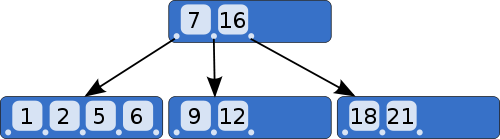
\includegraphics[width=.75\textwidth]{img/B-tree.png}
\caption[Beispiel für einen kleinen B-Baum]{Beispiel für einen kleinen B-Baum \footnotemark}
\label{bbaum}
\end{figure}
\footnotetext{Quelle: \cite{wmc} \url{http://commons.wikimedia.org/wiki/File:B-tree.svg}}
\\Der Vorteil des B-Baumes gegenüber dem Binärbaum ist, daß weniger Zugriffe auf den Massenspeicher notwendig sind, um zu einem Datensatz zu gelangen. Im schlechtesten Fall sind O(log(n)) Knoten zu durchsuchen. Wie auch beim Binärbaum ist beim B-Baum ein schneller Zugriff auf einen Bereich oder auf das Minimum bzw. Maximum der Daten möglich, da die Datensätze in einer definierten Ordnung abgelegt sind.

\subsubsection{Hashing}
Eine Methode um schnell auf einen Datensatz zuzugreifen ist das Hash-Verfahren. Hierbei wird der Schlüssel des Datensatzes mit einer Hash-Funktion auf eine RID abgebildet. Eine Hash-Funktion ist jedoch keine eineindeutige Abbildung, daher kann es auch zu Kollisionen kommen, mehrere Datensätze können also auf die gleiche RID abgebildet werden. In einem solchen Fall müssen dann weitere Mechanismen dafür sorgen, daß die Daten an einer anderen Stelle gespeichert und wieder aufgefunden werden können. Z.B. kann dies durch nochmalige Anwendung der Hash-Funktion erfolgen oder durch einen zusätzlichen Überlaufbereich, der die Daten einfach sequentiell speichert. Damit es möglichst selten zu Kollisionen kommt und der Zugriff dadurch verlangsamt wird, muß der für die Daten reservierte Speicher groß genug gewählt werden  \footnote{vgl. \cite{Sauer1998}, S. 153f}.
\begin{figure}[h]
\begin{lstlisting}[basicstyle=\ttfamily\scriptsize\singlespacing, commentstyle=,language=]
  |Kdnr | Name    |                        | RID  |Kdnr | Name    |
  |-----|---------|                        |------|-----|---------|
  | 123 | Bayer   |                        | 1000 |     |         |
  | 124 | Schmidt |      hash(Kdnr)=RID    | 1001 | 156 | Huber   |
  | 125 | Bauer   |  ------------------->  | 1002 | 125 | Bauer   |
  | 133 | Schulz  |                        |  .   |     |         |
  | 156 | Huber   |                        | 1250 | 123 | Bayer   |
                                           |  .   |     |         |
                                           | 2590 | 133 | Schulz  |
                                           | 3003 | 124 | Schmidt |
\end{lstlisting}
\caption[Abbildung von Datensätzen auf Hash-Adressen]{Abbildung von Datensätzen auf Hash-Adressen \footnotemark}
\label{hash}
\end{figure}
\footnotetext{eig. Darst. in Anlehnung an \cite{Sauer1998}, S. 153}
Der Vorteil des Hashing besteht darin, daß die Zugriffszeit nahezu unabhängig von der Tabellengröße ist (jedoch abhängig vom Füllgrad). In der Regel kann mit einem oder zwei Datenträgerzugriffen der Datensatz gefunden werden.
Der größte Nachteil ist die fehlende Sortierung der Daten. Bei einem Zugriff auf einen Bereich (WHERE Name LIKE 'B\%') muß die gesamte Tabelle durchsucht werden. Außerdem wird immer ein gewisser Teil des Speicherplatzes verschwendet.

\subsubsection{Heap} 
Bei einem Heap (deutsch: Haufen, Halde) werden alle Datensätze einfach der Reihe nach auf dem Datenträger abgelegt. Um auf einen bestimmten Datensatz zuzugreifen, muß daher u.U. der gesamte Heap gelesen werden. Dies ist bei großen Tabellen in der Regel ungünstig, kann jedoch eine Möglichkeit für kleinere Tabellen sein, die einen Umfang von einigen wenigen Speicherseiten haben, da diese komplett in den Datencache passen oder ggf. mit nur einem Datenträgerzugriff gelesen werden können.

\subsection{Abarbeitung von SQL-Ausdrücken}
Als Programmiersprache gehört SQL zu den 4GL-Sprachen. Das bedeutet, im Gegensatz zu den Programmiersprachen der 3. Generation wird nicht beschrieben WIE ein Ergebnis ermittelt werden soll, sondern WELCHES Ergebnis ermittelt werden soll. Das Problem wird bei SQL also auf einem anderen semantischen Level beschrieben. Intern muß jedoch die Abfrage wieder in einen linearen Programmcode umgewandelt werden, der von der CPU bearbeitet werden kann. Dies resultiert dann in mehr oder weniger verschachtelten Schleifen, je nach Anzahl der Tabellen, die miteinander verknüpft werden. Sind mehrere Tabellen in die Abfrage involviert, so muß das RDBMS deren karthesisches Produkt bilden, um dann das Ergebnis gemäß der Bedingungen in der WHERE-Klausen einzuschränken. Wenn auf die verknüpften Spalten nicht über Indizes zugegriffen werden kann, dann müssen tatsächlich alle möglichen Kombinationen geprüft werden.

\section{MySQL-EXPLAIN}
In vielen RDBMS steht mit dem SQL-Kommando EXPLAIN ein Werkzeug zur Verfügung, um mehr darüber zu erfahren, wie die Datenbank eine bestimmte Anfrage ausführt, wie also der Query Execution Plan (QEP) ist. Das EXPLAIN-Kommando gehört jedoch nicht zum SQL-Standard und wird bei den verschiedenen RDBMS unterschiedliche Ausgaben erzeugen. Bei MySQL ist EXPLAIN sehr mächtig und gibt umfassend und detailliert Auskunft über den QEP. Hierbei muß jedoch beachtet werden, daß der QEP nicht fix ist, sondern bei jeder Anfrage vom Optimierer erneut erstellt wird (sofern die Anfrage nicht bereits aus dem Query-Cache bedient werden kann). Es gibt daher keine Garantie, daß die Anfrage immer mit dem vorher von EXPLAIN gezeigten QEP ausgeführt wird. Es empfielt sich deswegen, die untersuchten SQL-Anfragen von Zeit zu Zeit erneut mit EXPLAIN zu prüfen.

\subsection{Umschreiben von Nicht-SELECT-Anfragen}
Vor MySQL 5.6.3 konnte EXPLAIN nur auf SELECT-Anfragen angewendet werden. \footnote{\cite{manual} \url{http://dev.mysql.com/doc/refman/5.6/en/using-explain.html}}
Einige Nicht-SELECT-Anfragen, wie DELETE, INSERT, REPLACE und UPDATE können jedoch in ein entsprechendes SELECT-Kommando umgeformt werden, um dieses dann mit EXPLAIN zu untersuchen. Zu beachten ist aber, daß schreibende Anweisungen generell aufwendiger sind als das entsprechende SELECT-Kommando, da zusätzlich zum Auffinden der Daten noch die Schreiboperation ausgeführt werden muß, ggf. kommen auch noch Aktualisierungen von Indizes hinzu. Z.B  kann {\tt DELETE user WHERE lastlogin < 2012-01-01} umgeformt werden zu {\\tt SELECT id FROM user WHERE lastlogin < 2012-01-01}

\subsection{Einfache SELECT-Anfragen mit einer Tabelle}
An einem Beispiel einer einfachen SELECT-Anfrage soll gezeigt werden, wie die Ausgabe einer EXPLAIN-Anweisung aufgebaut ist.
Hierzu wird zur Demonstation zuerst eine Tabelle mit einigen Daten erzeugt:
\begin{lstlisting}[caption=Anlegen einer Tabelle mit Wörtern]
mysql> CREATE TABLE words ( 
       id INT UNSIGNED AUTO_INCREMENT PRIMARY KEY, 
       word VARCHAR(60) ) ENGINE=InnoDB; 
-- Worte aus Wörterbuch in die Tabelle laden
mysql> LOAD DATA LOCAL INFILE '/usr/share/dict/ngerman'
       INTO TABLE words (word);
Query OK, 339099 rows affected (6,58 sec)
\end{lstlisting}
Es wurden also 339099 Zeilen bzw. Wörter in die Tabelle importiert, die id-Spalte hat MySQL dabei automatisch gefüllt und hochgezählt.
Nun sollen beispielhaft die fünf alphabetisch letzten Worte abgefragt werden:\\
\begin{minipage}{\linewidth}
\begin{lstlisting}[caption=Einfaches SELECT ohne Indexzugriff]
mysql> SELECT word FROM words ORDER BY word DESC LIMIT 5;
+-----------+
| word      |
+-----------+
| zzgl      |
| Zysten    |
...
5 rows in set (0,20 sec)
\end{lstlisting}
\end{minipage}

Durch Voranstellen von EXPLAIN läßt sich der QEP der Anfrage anzeigen:
\begin{lstlisting}[basicstyle=\ttfamily\scriptsize,caption=EXPLAIN mit einfachem SELECT]
mysql> EXPLAIN SELECT word FROM words ORDER BY word DESC LIMIT 5;
+----+-------------+-------+------+---------------+------+---------+------+--------+----------------+
| id | select_type | table | type | possible_keys | key  | key_len | ref  | rows   | Extra          |
+----+-------------+-------+------+---------------+------+---------+------+--------+----------------+
|  1 | SIMPLE      | words | ALL  | NULL          | NULL | NULL    | NULL | 341202 | Using filesort |
+----+-------------+-------+------+---------------+------+---------+------+--------+----------------+
\end{lstlisting}
Wie man erkennt, wurde das EXPLAIN-Kommando schneller ausgeführt als das eigentliche SELECT.
Dies liegt daran, daß EXPLAIN nicht tatsächlich auf die Daten in der Tabelle zugreift, sondern nur aufzeigt, wie die Datenbank die Datensätze auffinden würde.

\subsection{Die Spalten der EXPLAIN-Ausgabe}
Als Ergebnis einer EXPLAIN-Anfrage liefert MySQL eine Tabelle mit festen Spalten und einer oder mehrerer Zeilen, je nach Komplexität der Anfrage. Die einzelnen Spalten haben folgende Bedeutung  \footnote{vgl. \cite{manual} \\ \url{http://dev.mysql.com/doc/refman/5.6/en/explain-output.html},\\ \cite{Schwartz2009} S. 665-676, \\ \cite{Bradford2011} Pos. 2696-2906}:\\
\textbf{id}: identifiziert das SELECT, zu dem die Zeile gehört, bei einer einfachen SELECT-Abfrage stets die Zahl 1\\
\textbf{select\_type}: gibt an, ob es sich um ein einfaches oder komplexes SELECT handelt. Folgende Werte können auftreten:
\begin{description}[labelwidth=90pt,font=\ttfamily]
	\item[SIMPLE] einfaches SELECT, keine Unterabfragen oder UNIONS
	\item[PRIMARY] äußeres SELECT eines komplexen SELECT
	\item[SUBQUERY] SELECT in einer Unterabfrage
	\item[DERIVED] SELECT in einer Unterabfrage in der FROM-Klausel
	\item[UNION] zweites bzw. nachfolgende SELECT eines UNION
	\item[UNION RESULT] Ergebnis des UNION, wird aus temporärer Tabelle geholt
\end{description}
\textbf{table}: gibt an, auf welche Tabelle zugegriffen wird. Dies kann der tatsächliche Tabellenname sein oder der Alias. Die Spalte ist von oben nach unten zu lesen, um die Join-Reihenfolge zu sehen, die der Optimierer für die Anfrage gewählt hat.
Bei komplexeren Anfragen mit abgeleiteten Tabellen und Vereinigungen können hier noch weitere Werte auftreten: <derivedN> wenn es in der FROM-Klausel eine Unterabfrage gibt, wobei N die ID der Unterabfrage ist und in den nachfolgenden Zeilen der Ausgabe zu finden ist. Bei einer Vereinigung mit UNION enthält die UNION RESULT-Zeile in der table-Spalte die IDs der Abfragen, welche vereinigt werden, und beziehen sich daher immer auf vorhergehende Zeilen der Ausgabe, z.B. <union2,4>\\
\textbf{type}: Zugriffstyp, mit dem die Zeilen in der Tabelle aufgefunden werden. Folgende Werte können auftreten (in geordneter Reihenfolge vom langsamsten zum schnellsten Zugriffstyp):
\begin{description}[font=\ttfamily]
\item[ALL] full Tablescan, d.h., Tabelle muß in der Regel von Anfang bis Ende durchlaufen werden, ist ein starkes Indiz für weiteren Optimierungsbedarf
\item[index] wie Tablescan, aber Scannen der Tabelle erfolgt in Indexreihenfolge, eine extra Sortierung wird hierbei vermieden
\item[range] Bereichsscan, d.h., eingeschränkter Indexscan, z.B. bei BETWEEN oder > in der WHERE-Klausel
\item[ref] Index-Lookup findet statt, ein nichteindeutiger Index wird hierbei mit einem Referenzwert verglichen, die gefundenen Zeilen entsprechen dem Referenzwert, Variante: ref\_or\_null
\item[eq\_ref] Index-Lookup mit eindeutigem Treffer, bei Primärschlüssel oder eindeutigem Index
\item[const,system] der Datenzugriff konnte von MySQL wegoptimiert oder in eine Konstante umgewandelt werden.
\item[NULL] Abfrage kann von MySQL bei der Optimierung aufgelöst werden, kein Zugriff auf Tabelle oder Index, z.B. Minimum einer indizierten Spalte
\end{description}
\textbf{possible\_keys}: gibt an, welche Indizes für die Bearbeitung der Anfrage prinzipiell zur Verfügung stehen.
Die hier stehenden Werte werden bereits in einer frühen Phase der Optimierung ermittelt. Letzendlich wird in der Regel nur ein Index genutzt. Sind hier viele Indizes aufgeführt deutet das auf ein Problem hin.\\
\textbf{key}: key gibt an, welchen Index der Optimierer für die Anfrage gewählt hat. Dies kann auch ein abdeckender Index sein, aus dem die Ergebniswerte gelesen werden können, ohne daß die eigentliche Tabelle gelesen werden muß. Ein Wert von NULL in der Spalte key bedeutet, daß kein Index genutzt wird und ist ein starkes Indiz für einen Optimierungsbedarf.\\
\textbf{key\_len} gibt an, wieviel Byte (Spaltenbreite) eines Index benutzt werden. Die Zählung beginnt links, man kann so ermitteln, welche Spalten des Index genutzt werden.\\
\textbf{ref}: gibt an, welche Spalten aus früheren Tabellen benutzt werden, um in dem key-Index nachzuschlagen.\\
\textbf{rows}: Zahl ist eine Schätzung für die Anzahl der Zeilen, die gelesen werden müssen.
Bei Abfragen mit mehreren Tabellen gilt diese Angabe pro Schleifendurchlauf im Nested-Loop-Join-Plan.
Die Schätzung beruht auf Statistiken und kann ungenau sein. Im besten Fall steht hier eine 1.\\
\textbf{Extra} enthält weitere Angaben, die nicht in die anderen Spalten passen:
\begin{description}[font=\ttfamily]
\item[Using Index] abdeckender Index wird genutzt, d.h., die angefragten Daten müssen nicht aus der Tabelle gelesen werden
\item[Using where] die Zeilen werden nachträglich gefiltert, d.h., für die WHERE-Bedingung wird nicht der Index genutzt
\item[Using temporary] Erstellung einer temporären Tabelle für Sortierung 
\item[Using filesort] externe Sortierung, im RAM oder auf dem Datenträger
\item[ranke checked for each record (index map: N)] kein geeigneter Index vorhanden, N ist ein Bitmap auf die Spalten in possible\_keys
\end{description}
\subsubsection{EXPLAIN EXTENDED}
Wird EXPLAIN EXTENDED anstatt von EXPLAIN verwendet, dann erscheint seit MySQL 5.1 die zusätzliche Spalte \textbf{filtered}. Es handelt sich um eine pessimistische Schätzung des Prozentsatzes der Zeilen, die eine Bedingung erfüllen, wie z.B. eine WHERE-Klausel oder ein JOIN mit einer anderen Tabelle.
Außerdem werden weitere Informationen generiert, die mit dem nachfolgenden SQL-Kommando SHOW WARNINGS angezeigt werden können.  \footnote{\cite{manual} \url{http://dev.mysql.com/doc/refman/5.6/en/explain-extended.html}}.
\subsubsection{EXPLAIN PARTITIONS}
Wird EXPLAIN PARTITIONS verwendet, dann zeigt die zusätzlichen Spalte \textbf{partitions} die Partitionen, auf welche die Anfrage zugreift, sofern welche verfügbar sind. Diese Option ist erst seit MySQL 5.1 verfügbar.
Das Schlüsselwort EXTENDED kann nicht zusammen mit EXPLAIN PARTITIONS verwendet werden.
\subsection{Abfragen mit mehreren Tabellen}
Vor allem bei Anfragen, die mehrere Tabellen verbinden, kann EXPLAIN interessante Informationen liefern. Häufig sind es gerade diese Anfragen, die sehr aufwendig sind und den DB-Server beanspruchen.
Zur Demonstration wird zuerst eine weitere einfache Tabelle angelegt und mit Primzahlen aus einer Datei gefüllt:
\begin{lstlisting}[caption=Anlegen einer primitiven Tabelle mit Primzahlen]
-- # primes 1 100000000 > /tmp/primes
-- # sudo chown mysql:mysql /tmp/primes
mysql> CREATE TABLE big ( p INT NOT NULL );
mysql> LOAD DATA INFILE "/tmp/primes" into table big;
>Query OK, 5761455 rows affected (49,15 sec)
\end{lstlisting}
Diese soll nun mit der Tabelle \textbf{words} verknüpft werden, um die (alphabetisch sortierten) ersten fünf Worte auszugeben, welche eine Primzahl als id haben.\\
\begin{minipage}{\linewidth}
\begin{lstlisting}[caption=Abfrage von zwei verknüpften Tabellen (Join)]
mysql> SELECT p,word FROM words, big WHERE p=id ORDER BY word LIMIT 5;
+--------+---------------+
| p      | word          |
+--------+---------------+
|     29 | Aachener      |
|     31 | Aachenerinnen |
...
5 rows in set (22,67 sec)
\end{lstlisting}
\end{minipage}
\\Mit über 22 Sekunden Laufzeit war diese relativ simple Anfrage für den Datenbank-Server sehr aufwendig.
Mit EXPLAIN zeigt sich, warum die Ausführung der Anfrage so aufwendig war:
\begin{lstlisting}[basicstyle=\ttfamily\tiny,caption=Ausführungsplan ohne Optimierung]
mysql> EXPLAIN SELECT p,word FROM words, big WHERE p=id ORDER BY word LIMIT 5;
+----+-------------+-------+--------+---------------+---------+---------+-----------------+---------+---------------------------------+
| id | select_type | table | type   | possible_keys | key     | key_len | ref             | rows    | Extra                           |
+----+-------------+-------+--------+---------------+---------+---------+-----------------+---------+---------------------------------+
|  1 | SIMPLE      | big   | ALL    | NULL          | NULL    | NULL    | NULL            | 5672186 | Using temporary; Using filesort |
|  1 | SIMPLE      | words | eq_ref | PRIMARY       | PRIMARY | 4       | primetest.big.p |       1 | Using where                     |
+----+-------------+-------+--------+---------------+---------+---------+-----------------+---------+---------------------------------+
\end{lstlisting}
Beide Zeilen haben die id 1, denn es handelt sich nur um ein SELECT. Die erste Zeile bezieht sich auf die Tabelle \textbf{big}. Diese Tabelle hat keinen Primärschlüssel und auch keinen anderen Index (possible\_keys=NULL, key=NULL). Daher muss sie komplett durchlaufen werden (type=ALL, rows=5672186). Außerdem wird die Tabelle auch noch nach dem kompletten Lesen sortiert (Extra=Using filesort). Dies alles ist für die Datenbank sehr aufwendig. Die zweite Zeile bezieht sich auf die Tabelle \textbf{words}. Hier kann der Zugriff über den Primärschlüssel erfolgen (key=PRIMARY), welcher ja immer UNIQUE ist. Von der Tabelle \textbf{words} wird deshalb pro gelesener Zeile von Tabelle \textbf{big} nur eine Zeile gelesen (rows=1). Allerding werden über 5 Mio. Zeilen von \textbf{big} gelesen.
\subsection{Optimierungsmöglichkeiten und Benchmarking}
Bevor man die Datenbank optimiert und die SQL-Anfragen benchmarkt sollte man sicherstellen,
daß der Query-Cache von MySQL nicht aktiv ist (query\_cache\_type=OFF und query\_cache\_size=0). MySQL kann sonst bei unverändertem SQL die Anfragen direkt aus dem Query-Cache bedienen.\footnote{vergl. \cite{Kraze2011}} Für die Optimierung sind die wichtigsten Spalten der EXPLAIN-Ausgabe \textbf{key} (benutzer Index), \textbf{rows} (Anzahl Zeilen bearbeitet) und \textbf{type} (Zugriffstyp).
Bei dem oben genannten Beispiel kann man anhand dieser drei Spalten erkennen, daß der Zugriff auf die Primzahlen langsam ist, weil kein Primärschlüssel oder ein anderer Index existiert.
Für einen neu anzulegenden Index kann hier das Schlüsselwort UNIQUE verwendet werden, da keine Zahl mehrfach in der Tabelle vorkommen kann:
\begin{lstlisting}[caption=1. Optimierung: Anlegen eines Index für die Primzahlen]
mysql> ALTER TABLE big ADD UNIQUE INDEX IX_P USING BTREE (p ASC);
Query OK, 0 rows affected (48,53 sec)
\end{lstlisting}
Man sieht, daß das Anlegen eines Index recht lange dauern kann. Die Tabelle wird für diesen Zeitraum für Schreibzugriffe gesperrt. Auf einem Produktiv-System ist daher mit großer Vorsicht und gründlicher Planung zu agieren, vorher sollte man sich Informationen über die Größe der Tabelle holen und am besten einen Probedurchlauf auf einer Kopie der Tabelle machen!
Doch welche Auswirkung hat das Anlegen des Index auf die SQL-Anfrage?
\begin{lstlisting}[caption=Abfrage nach 1. Optimierung]
mysql> SELECT p,word FROM words, big WHERE p=id ORDER BY word LIMIT 5;
5 rows in set (0,46 sec)
\end{lstlisting}
Die Abfrage hat sich von 22,67s auf 0,45s reduziert, also um Faktor 49!
\begin{lstlisting}[basicstyle=\ttfamily\tiny, caption=Ausführungsplan nach 1. Optimierung]
mysql> EXPLAIN SELECT p,word FROM words, big WHERE p=id ORDER BY word LIMIT 5;
+----+-------------+-------+--------+---------------+------+---------+--------------------+--------+--------------------------+
| id | select_type | table | type   | possible_keys | key  | key_len | ref                | rows   | Extra                    |
+----+-------------+-------+--------+---------------+------+---------+--------------------+--------+--------------------------+
|  1 | SIMPLE      | words | ALL    | PRIMARY       | NULL | NULL    | NULL               | 341202 | Using filesort           |
|  1 | SIMPLE      | big   | eq_ref | IX_P          | IX_P | 4       | primetest.words.id |      1 | Using where; Using index |
+----+-------------+-------+--------+---------------+------+---------+--------------------+--------+--------------------------+
\end{lstlisting}
Die Reihenfolge, in welcher die Tabellen gelesen werden hat sich jetzt umgekehrt.
Auf die Tabelle mit den Primzahlen kann nun über den Index zugegriffen werden, es kann sogar direkt aus dem abdeckenden Index gelesen werden (Extra=Using index), ohne auf die eigentliche Tabelle zugreifen zu müssen. Jedoch wird jetzt auf der Wörter-Tabelle ein full Tablescan ausgeführt und über 300.000 Zeilen müssen gelesen werden, denn die Worte müssen weiterhin nachträglich sortiert werden (Extra=Using filesort).
Mit einem weiteren Index auf die Spalte word lässt sich das Sortierungsproblem lösen:
\begin{lstlisting}[caption=2. Optimierung: Anlegen eines Index für die Wörter]
mysql> ALTER TABLE words ADD INDEX IX_WORD USING BTREE (word ASC);
Query OK, 0 rows affected (2,06 sec)
\end{lstlisting}
UNIQUE INDEX läßt sich hier nicht anwenden, da ein Wort mehrfach vorkommen kann.
Mit dem neuen Wörter-Index hat sich die Zeit noch einmal verbessert:
\begin{lstlisting}[caption=Abfrage nach 2. Optimierung]
mysql> SELECT p,word FROM words, big WHERE p=id ORDER BY word LIMIT 5;
5 rows in set (0,00 sec)
\end{lstlisting}
Die Abfragezeit ist nun kleiner als 10 ms, laut Workbench sogar unter 1ms! Der optimierte QEP ist nun folgender:
\begin{lstlisting}[basicstyle=\ttfamily\tiny,caption=Ausführungsplan nach 2. Optimierung]
mysql> EXPLAIN SELECT p,word FROM words, big WHERE p=id ORDER BY word LIMIT 5;
+----+-------------+-------+--------+---------------+---------+---------+--------------------+------+--------------------------+
| id | select_type | table | type   | possible_keys | key     | key_len | ref                | rows | Extra                    |
+----+-------------+-------+--------+---------------+---------+---------+--------------------+------+--------------------------+
|  1 | SIMPLE      | words | index  | PRIMARY       | IX_WORD | 63      | NULL               |    5 | Using index              |
|  1 | SIMPLE      | big   | eq_ref | IX_P          | IX_P    | 4       | primetest.words.id |    1 | Using where; Using index |
+----+-------------+-------+--------+---------------+---------+---------+--------------------+------+--------------------------+
\end{lstlisting}
Jetzt können auch die Worte aus dem abdeckenden Index gelesen werden. Es müssen nur 5 Zeilen aus der Wörtertabelle und jeweils 1 Zeile aus der Primzahlentabelle gelesen werden
Insgesamt werden also nur 10 Datensätze direkt aus dem Index gelesen, und zwar genau die Daten, die auch ausgegeben werden sollen.
\\An diesem einfachen Beispiel zeigt sich, wie mit Hilfe von Explain und Anlegen der richtigen Indizes die Performance von Abfragen um Größenordnungen gesteigert werden kann.
\\Wird ein vorhandener Index bei der Anfrage nicht genutzt, obwohl er augenscheinlich genutzt werden sollte, dann kann das an veralteten Tabellen-Statistiken oder einer ungenügenden Stichprobe für die Statistiken liegen. Die Statistiken für eine Tabelle lassen sich dann mit ANALYZE TABLE Tabellenname aktualisieren.\footnote{vergl. \cite{Erk2008}}
\\Als Nachteil von Indizes ist anzumerken, daß bei Schreibzugriffen auf die Tabelle ein gewisser Mehraufwand für die Datenbank besteht, da neben der Tabelle auch der Index aktualisiert werden muß. Bei Tabellen, in welche ständig sehr viel geschrieben wird, z.B. für Logging-Zwecke, könnten Indizes daher nachteilig sein.
Einige weitere wichtige Punkte für die Datenbank-Optimierungen seien noch genannt:\footnote{vergl. \cite{Galperin2011}}
\begin{itemize} 
	\item möglichst zuerst den Programmcode der Anwendung optimieren, um DB-Anfragen zu bündeln (1+n-Problem)
	\item bereits im Entwicklungsprozeß die DB-Anfragen proaktiv beobachten
	\item mit verschiedenen Beispielwerten testen - der QEP ist nicht fix, sondern wird bei jeder Abfrage neu erstellt
	\item nicht mit Entwicklungs-Datenbanken (kaum gefüllte Tabellen) testen, sondern Real-Word-Daten einsetzen, z.B. aus Backups
	\item auf Produktiv-Systemen mit einer Stichprobe (z.B. jede 100. Anfrage) benchmarken - Systeme unter Last agieren anders als Systeme im Leerlauf
	\item Tests von Zeit zu Zeit wiederholen, da sich die Tabellen im Laufe des Betriebs weiter füllen
\end{itemize}
\section{Fazit und Ausblick}
Es wurde gezeigt, wie ein RDBMS mit Hilfe von Indizes schneller auf Daten zugreifen kann.
Exemplarisch wurde für MySQL ein Workflow demonstriert, mit dem mittels EXPLAIN SQL-Anfragen um mehrere Größenordnungen beschleunigt werden konnten.
Hierbei ist zu beachten, daß EXPLAIN keine exakten Angaben liefert, daher ist immer auch eine Überprüfung der Optimierung mit Benchmarks notwendig.
Aus Platzgründen konnte leider auf viele weitere Möglichkeiten der Datenbank-Optimierung nicht eingegeangen werden, wie Umschreiben von ungünstigen SQL-Anfragen, Nutzung des Query-Caches, Profiling der Datenbank, Profiling der Anwendung, Eleminierung überflüssiger Indizes, Eleminierung überflüssiger Datenspalten in der SQL-Anfrage. 
Es wurden auch nur relativ einfache SELECT-Anfragen untersucht, keine UNIONS, oder Subselects.
Dies alles wären Themen für weitergehende Arbeiten.
